\documentclass[numbers=endperiod, 11pt]{scrartcl}
\usepackage[left=1.1in,right=1.1in]{geometry}
\usepackage[secthm,mdthm]{evan}
\usepackage[most]{tcolorbox}
\usepackage{cancel}
\usepackage[labelfont=bf,sf, font=sf]{caption}
\usepackage{bm}

\setcounter{section}{-1}

\addtokomafont{paragraph}{\color{DeepSkyBlue!35!black}\P\,}
% \setparsizes{20pt}{4pt}{0pt plus 1fil}

\newcommand{\bsquare}{\hfill$\blacksquare$\par\medskip}
\newenvironment{sol}{%
     \par\medskip\noindent\textit{Solution.}}{%
     \hfill$\blacksquare$\par\medskip}

\newtcbtheorem[auto counter]{prob}{\textbf{Problem}}%
    {enhanced,frame empty,interior empty, sharp corners, colframe=magenta, top=1.5mm,separator sign none, coltitle=white,fonttitle=
    \sffamily \bfseries, description font=\mdseries\sffamily, colbacktitle=magenta!100!white,
        borderline={0.5mm}{0mm}{magenta!15!},
        borderline={0.5mm}{0mm}{magenta!100!white},
        attach boxed title to top left={yshift=0mm},
        boxed title style=sharp corners,
    }{thm} %(description font helps in resolving issues with theorem name and custom theorem name as fonttitle gives same font family to both Theorem name and Number)

\makeatletter
\renewcommand*{\eqref}[1]{%
  \hyperref[{#1}]{\textup{\tagform@{\ref*{#1}}}}%
}
\makeatother

\ihead{\textbf{Pragyan Pranay} (last updated \today)}
\ohead{\footnotesize\url{satisfiedmagma.github.io}}

\begin{document}
\title{ISI UGB 2026 Solutions}
\subtitle{Unofficial Solutions of UGB Paper}
\author{Pragyan Pranay}
\date{11 June, 2026}
\maketitle

\begin{abstract}
    These are unofficial solutions to ISI Entrance UGB
	Paper, 2026. The main motivation of writing these
	solutions is the absencse of any official solutions
	on the internet and to help the students with the
	technical details of proof-writing in a proof-based
	mathematical setting.
\end{abstract}

The tone of the solutions given here is very dry and
very much to the point and I more or less expect a student
to have certain mathematical maturity.

I understand that for some people these problems could
be hard and quite unconventional. Keeping this in mind, I've
not only put out the solution, but I've also written a blog
post at
\begin{center}
    \small
    \url{https://satisfiedmagma.github.io/writings/posts/isi_2026_discussion/}
\end{center}

\noindent which doesn't have formal solutions, but rather
an interesting commentary and the thought process to solve
these problems. I agree that not everything can be motivated;
a few techniques must be known beforehand but I've tried
my best to put my thoughts on the blog as naturally and
as clearly as possible.

\tableofcontents
\newpage

\section{Problems}

\begin{enumerate}
    \item The problem is in two parts.
          \begin{enumerate}
              \item Let $a, b \in \RR$ be such that
                    the straight line $y = a + bx$ on the
                    $(x, y)$-plane passes through
                    $(x_1, y_1)$ and $(x_2, y_2)$. If
                    $x_1, y_1, x_2, y_2$ are rational
                    numbers with $x_1 \neq x_2$ and
                    $y_1 \neq y_2$, show that $a$ and $b$ are
                    rational numbers and $b \neq 0$.
              \item Let $\alpha, \beta, r \in \RR$ be such
                    that $r > 0$ and the circle
                    $(x - \alpha)^2 + (y - \beta)^2 = r^2$ on
                    the $(x, y)$-plane passes through
                    $(x_1, y_1)$, $(x_2, y_2)$ and
                    $(x_3, y_3)$. Assume that $x_1, x_2, x_3$
                    are distinct rational numbers and
                    $y_1, y_2, y_3$ are distinct rational
                    numbers. Show that $\alpha$ and $\beta$
                    are rational numbers.
          \end{enumerate}

    \item Sketch with reasoning, the graph of
          $y = (\log_e x)^2 + (\log_e x)^{-2}$.

    \item Suppose $n \geq 2$ is an integer. Define
          \[S = \{(x_1, \dots, x_n) : 0 < x_i < 1 \text{ for all } i = 1, \dots, n\}\]
          and a function $f\colon S \to \RR$ by
          \[f(x_1, \dots, x_n) = \log_{x_1} ((x_2)^2) + \dots + \log_{x_{n-1}} ((x_n)^n) + \log_{x_n} x_1.\]
          Determine the minimum value of
          $f(x_1, \dots, x_n)$ over $S$.

    \item Suppose $f\colon \RR \to \RR$ is a twice
          differentiable function such that
          \[f(x + y) + f(x - y) = 2(f(x) + f(y)) \text{ for all } x, y \in \RR.\]
          \begin{enumerate}
              \item If $f'$ denotes the derivative of $f$,
                    show that
                    \[f'(x + y) - f'(x - y) = 2f'(y) \text{ for all } x, y \in \RR.\]
              \item Further assume that $f''(0) = 2$, where
                    $f''$ is the second derivative of $f$.
                    Determine $f$.
          \end{enumerate}

    \item In the figure below, $ABCD$ is a square. The
          points $E, F, G, H$ lie on $AB, BC, CD, DA$,
          respectively, such that $EFGH$ is a square. The
          perimeter of $ABCD$ exceeds the perimeter of
          $EFGH$ by 32 units. Determine the length of the
          radius of the in-circle of $\Delta EBF$.
          \begin{figure}[ht]
              \centering
              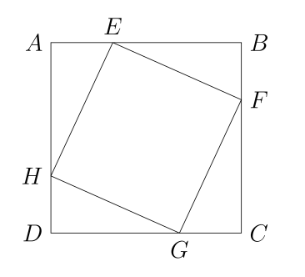
\includegraphics[scale=0.6]{../../../src/content/posts/isi_2026_discussion/geo_question.png}
          \end{figure}

    \item Let $P$ be a polynomial of degree greater than or
          equal to one, with real coefficients, such that
          $P(x) \geq 0$ for all $x \in \RR$.
          \begin{enumerate}
              \item Suppose $x_0 \in \RR$ is such that
                    $P(x_0) = 0$. Show that there exist a
                    positive integer $n$ and a polynomial
                    $S$ with real coefficients such that
                    $S(x_0) \neq 0$ and
                    \[P(x) = (x - x_0)^{2n} S(x) \text{ for all } x \in \RR.\]
              \item Hence or otherwise, show that there
                    exist polynomials $Q$ and $R$ with real
                    coefficients such that $R(x) > 0$ for
                    all $x \in \RR$ and
                    \[P(x) = (Q(x))^2 R(x) \text{ for all } x \in \RR.\]
          \end{enumerate}
    \item Suppose $P$ is a polynomial with integer
          coefficients.
          \begin{enumerate}
              \item Show that for distinct integers $m$ and
                    $n$, $\frac{P(m) - P(n)}{m - n}$ is an
                    integer.
              \item Hence or otherwise, prove that there do
                    not exist distinct integers $a, b, c$
                    such that
                    \[P(a) = b, \quad P(b) = c, \quad \text{and} \quad P(c) = a.\]
          \end{enumerate}
    \item Let $k$ be a non-negative integer.
          \begin{enumerate}
              \item Show that there exists a unique
                    polynomial $P_k$ of degree $k+1$ with
                    real coefficients such that
                    \[\sum_{i=1}^{n} i^k = P_k(n) \text{ for all } n \geq 1.\]
              \item Determine the coefficient of
                    $x^{k+1}$ in $P_k(x)$.
              \item Hence or otherwise, determine the
                    coefficient of $x^k$ in $P_k(x)$.
          \end{enumerate}
\end{enumerate}
\newpage

\section{UGB 2026/1}

\begin{prob}{(UGB 2026/1)}{}
    The problem is in two parts.
    \begin{enumerate}[label=\alph*)]
        \item Let $a, b \in \RR$ be such that
              the straight line $y = a + bx$ on the
              $(x, y)$-plane passes through
              $(x_1, y_1)$ and $(x_2, y_2)$. If
              $x_1, y_1, x_2, y_2$ are rational
              numbers with $x_1 \neq x_2$ and
              $y_1 \neq y_2$, show that $a$ and $b$ are
              rational numbers and $b \neq 0$.
        \item Let $\alpha, \beta, r \in \RR$ be such
              that $r > 0$ and the circle
              $(x - \alpha)^2 + (y - \beta)^2 = r^2$ on
              the $(x, y)$-plane passes through
              $(x_1, y_1)$, $(x_2, y_2)$ and
              $(x_3, y_3)$. Assume that $x_1, x_2, x_3$
              are distinct rational numbers and
              $y_1, y_2, y_3$ are distinct rational
              numbers. Show that $\alpha$ and $\beta$
              are rational numbers.
    \end{enumerate}
\end{prob}

\begin{sol}
    We will split the solutions into two parts.

    \paragraph{Solution to part a)} Since
    $(x_1,y_1)$ and $(x_2,y_2)$ lie on the line
    $y = a + bx$, upon substituting we get
    \begin{align*}
        y_1 & = a + bx_1  \\
        y_2 & = a + bx_2.
    \end{align*}
    Subtracting the above two equations, we get
    \[y_1 - y_2 = b(x_1 - x_2). \]
    Since we are given that $x_1 \ne x_2$, therefore we can
    divide by $x_1 - x_2$ to get
    \[ b = \frac{y_2 - y_1}{x_2 - x_1}. \]
    Since $y_2 - y_1 \in \QQ$ and $x_2 - x_1 \in \QQ$ with
    $x_2 - x_1 \ne 0$(since we are given $x_1 \ne x_2$),
    we can conclude that $b \in \QQ$ since quotient of two
    rational numbers is a rational. Finally, note that
    \[ y_1 - bx_1 = a \]
    and since $y_1, x_1 \in \QQ$ and we just proved
    $b \in \QQ$, we get that
    $a = y_1 - bx_1 \in \QQ$(since difference of two
    rationals is always rational)
    \textbf{finishing the proof to part a). \bsquare}

    \paragraph{Solution to part b)} To be added, for now
	visit the blog-post at
	\begin{center}
		\small
		\url{https://satisfiedmagma.github.io/writings/posts/isi_2026_discussion/#-problem-1}
	\end{center}
	to see a sketch of the proof. \textbf{Thank You!}

\end{sol}
\newpage

\section{UGB 2026/2}

\begin{prob}{(UGB 2026/2)}{}
    Sketch, with reasoning, the graph of
    $y = (\log_e x)^2 + (\log_e x)^{-2}$.
\end{prob}
\begin{sol}
    For the entire solution, we will denote $\log_e(x)$ as
    $\ln(x)$. Define $\RR_{>0}$ as set of positive reals.
    We will begin with the following simple observations.
    \begin{itemize}
        \item The \textbf{domain of expression} is
              $T \coloneqq \RR_{> 0} \setminus \{1\}$. So,
              define a function $f\colon T \to \RR$ such
              that
              \[ f(x) = (\ln x)^2 + \frac{1}{(\ln x)^2} \quad \text{for all }x \in T.\]
              We need to graph $f$.
        \item $f$ has \textbf{no real roots.} Indeed if
              $f(\alpha) = 0$ for some $\alpha \in T$, then
              \[ 0 \le (\ln \alpha)^2 = \frac{-1}{(\ln \alpha)^2} < 0 \]
              which is absurd.
        \item $f$ has \textbf{two vertical asymptotes},
              one with the line $x = 0$ and one with the line
              $x = 1$(note that $0,1 \not\in T$). Indeed,
              \[ \lim_{x \to 0^+} f(x) = \lim_{x \to 0^+} \left((\ln x)^2 + \frac{1}{(\ln x)^2}\right) = +\infty = \lim_{x \to 1^-} f(x) = \lim_{x \to 1^+} f(x).\]
              Any other line is not an asymptote since
              $f$ is a continuous function in its domain $T$.
    \end{itemize}

    We now analyze the derivative of $f$ to find
    nature of monotonicity of $f$ and find its local
    maxima/minima.

    \begin{claim*}
        The function $f$ is
        \begin{itemize}
            \item \textbf{strictly increasing} on $\displaystyle \left( \frac 1 e , 1 \right)$ and $(e,\infty)$;
            \item \textbf{strictly decreasing} on $\displaystyle \left( 0, \frac 1 e \right)$ and $(1,e)$.
        \end{itemize}
        Moreover, $f$ has a \textbf{local and a global
            minima} of $2$ at $x = e, \frac 1 e$.
    \end{claim*}
    \begin{proof}
        Since $f$ is differentiable everywhere in its
        domain. Differentiating $f$ with yields
        \[ f'(x) = \frac 2 x \left( \ln x - \frac{1}{(\ln x)^3} \right) \quad \text{for all }x \in T.\]
        Observe that
        \begin{align*}
            f'(x) > 0 \iff \frac 2 x \left(\ln x - \frac{1}{(\ln x)^3}\right) > 0                                     \\
            \iff \frac 2 x \left( \frac{(\ln x)^4 - 1}{(\ln x)^3} \right)\cdot \left( \frac x 2 (\ln x)^4 \right) > 0 \\
            \iff (\ln x)^3 \left( (\ln x)^4 - 1 \right) > 0                                                           \\
            \iff \ln x \in (-\infty, 0) \cup (1,\infty)                                                               \\
            \iff x \in \left( \frac 1 e , 1\right) \cup (e,\infty).
        \end{align*}
        Since the derivative is non-negative on
        $\left( \frac 1 e , 1 \right)$ and $(e,\infty)$,
        $f$ must be strictly increasing on those intervals
        and strictly decreasing on intervals
        $\left( 0, \frac 1 e \right)$ and $(1,e)$.
        \vspace{1.2mm}

        Further, its easy to see
        $f'(x) = 0 \iff x = e,\frac 1 e$. So, a local
        maxima/minima can only occur at $x = e$ or
        $x = \frac 1 e$. Since $f'(x) > 0$ for all
        $x > e$ and $f'(x) < 0$ for $x \in (1,e)$,
        by the \textbf{first-derivative test} of
        local minima at $x = e$, we get that $x = e$
        must be the point of local-minima. Similarly,
        $x = 1/e$ is also a point of local minima. Also,
        $f(e) = f(1/e) = 2$.

        By AM-GM Inequality,
        \[ f(x) = (\ln x)^2 + \frac{1}{(\ln x)^2} \ge 2\sqrt{(\ln x)^2 \cdot \frac{1}{(\ln x)^2}} = 2 \quad \text{for all } x \in T \]
        which shows that $2$ is indeed the
        \textbf{global minima} of $f$ which
        \textbf{proves our claim.}
    \end{proof}

    \paragraph{Curvature of $\bm{f}$} We wish to find
    when is $f$ convex and when is $f$ concave. We need a
    preparatory lemma to tackle this part.

    \begin{lemma*}
        Consider $h(x) \coloneqq x^5 - x^4 - x - 3$, then
        \[ h(x) > 0 \iff x > \beta\]
        where $1 < \beta < 2$.
    \end{lemma*}
    \begin{proof}
        Note that
        \[ h'(x) = 5x^4 - 4x^3 -1 = (x-1)(5x^3+x^2+x+1)\]
        For $x > 1$, $h'(x) > 0$. Thus $h$ is strictly
        increasing over $(1,\infty)$. Also,
        $h(1) < 0$ and $h(2) < 0$. By
        \emph{Intermediate Value Theorem}, there is
        some $\beta \in (1,2)$ such that $h(\beta) = 0$.
        Since $h$ is increasing on $(1,\infty)$, we get
        \[x > \beta > 1 \implies h(x) > h(\beta) = 0 \quad \text{for all }x > \beta. \]
        It is now sufficient to show that $h(x) < 0$
        for all $x < \beta$. Define
        $r(x) \coloneqq 5x^3 + x^2 + x + 1$. Then
        \[ r'(x) = 15x^2 + 2x + 1 \ge 2x^2 + 2x + 1 = (x+1)^2 + x^2 > 0\]
        which shows that $r$ is strictly increasing. Since
        $r$ is a cubic polynomial, it must have at least
        root(which will be the only root since $r$ is
        increasing) which we shall call $\alpha$. Then
        we can write $r(x) = (x-\alpha)P(x)$ where $P$
        must be a strictly positive quadratic polynomial.
        Once again, since $r(-1) = -4 < 0$ and $r(0) = 1$,
        by \emph{Intermediate Value Theorem},
        $-1 < \alpha < 0$. Thus,
        \[h'(x) = (x-\alpha)(x-1)P(x). \]
        This means $h$ is increasing over
        $(-\infty, \alpha)$ and $(1,\infty)$ and
        decreasing over $(\alpha, 1)$. We now prove the
        following claim.

        \begin{claim*}[Computer Sorcery]
            $h(x) < 0$ for all $x < 0$\footnote{Check out the \href{https://satisfiedmagma.github.io/writings/posts/isi_2026_discussion/}{blog here} to find the reason for the name of this claim!}.
        \end{claim*}
        \begin{proof}
            We will make two cases, whether
            $x \in (-\infty, -1)$ or $(-1,0)$ or $x = -1$.
            The case $x = -1$ can be just checked
            by hand.

            If $x < -1$, then $x^4 > 1 \iff x^4 - 1 > 0$.
            This gives $x(x^4-1) < 0$. Then
            \[
                h(x) = x^5 - x^4 - x - 3 = x(x^4-1) - (x^4 + 3) < -(x^4 + 3) < 0.
            \]

            This completes the proof to the first case. For
            the second case, assume $-1 < x < 0$. This
            gives $-2 < x-1 < -1$ and $-3 < -x - 3 < -2$.
            Then
            \[
                h(x) = x^5 - x^4 - x - 3 = x^4(x-1) - x - 3 < -x^4 - x - 3 < -x^4 - 2 < 0
            \]
            this concludes the proof.
        \end{proof}
        We now only need to show that $h(x) < 0$ for
        $0 < x < \beta$. We already know that $h$ is
        decreasing over $(0,1)$, which means
        \[0 < x < 1 \implies 0 > -3 = h(0) > h(x) \quad \text{for all } x \in (0,1).\]
        Since $h$ is increasing over $(1,\beta)$, we
        can similarly show that $h$ is negative over
        $(1,\beta)$ as well. The graph of $h$ is given
        below.

        \begin{figure}[ht]
            \centering
            \begin{asy}
                import graph;
                size(120, 250, IgnoreAspect);
                ngraph = 10000;

                real h(real x) { return x^5 - x^4 - x - 3; }

                draw(graph(h, -1.5, 2.2), linewidth(0.8) + deepgreen, ArcArrows);

                dot((0,-3));
                dot((1,-4));

                xaxis("$x$", -4.9, 3.9, Ticks(Label(fontsize(1)),Step=1, Size=2, NoZero), ArcArrows);
                yaxis("$y$", -16.9, 25.9, Ticks(Label(fontsize(1)),Step=2, Size=2, NoZero), ArcArrows);
            \end{asy}
            \caption{Rough Sketch of $h(x) = x^5 - x^4 - x - 3$}
        \end{figure}
        This indeed \textbf{completes the proof to this
            lemma.}
    \end{proof}

    To find the \emph{curvature} of $f$, we need to compute
    the double derivative of $f$. Once again, $f'$ is
    differentiable on $T$, thus we get
    \[ f''(x) = \frac{2}{x^2} \left(1 - \ln x + \frac{1}{(\ln x)^3} + \frac{3}{(\ln x)^4} \right) \]
    for all $x \in T$. Note that
    \[f''(x) > 0 \iff (\ln x)^5 - (\ln x)^4 - \ln x - 3 < 0   \iff h(\ln x) < 0, \quad \text{where $x > 0$ and $x \ne 1$}\]
    where we got the first iff condition by multiplying by
    $\frac{x^2}{2}\cdot (\ln x)^4 > 0$. Invoking
    our preparatory lemma, we get
    \[ f''(x) > 0 \iff h(\ln x) < 0 \iff \ln x \in (-\infty, \beta)\setminus \{0\} \]
    which gives
    \[f''(x) > 0 \iff x \in \left( \exp(-\infty), \exp(\beta)\right) \setminus \{e^0\} = (0,e^{\beta}) \setminus \{1\}. \]
    Thus, by the \textbf{double-derivative test} of
    convexity, $f$ is \emph{convex} over $(0,1)$ and
    $(1,e^\beta)$. Similarly, $f$ is \emph{concave} over
    $(e^\beta, \infty)$ where $1 < \beta < 2$. We now
    present two sketches of the graph, one is
    computer-generated and one is drawn by hand.

    \begin{figure}[ht]
        \centering
        \begin{minipage}{.5\textwidth}
            \centering
            \begin{asy}
                import cse5;
                import graph; size(200);
                ngraph = 10000;

                real labelscalefactor = 0.5; /* changes label-to-point distance */
                pen dps = linewidth(0.7) + fontsize(11); defaultpen(dps); /* default pen style */
                pen dotstyle = black; /* point style */
                real xmin = -1, xmax = 11, ymin = -1, ymax = 8.5;

                pen qqwuqq = rgb(0.,0.39215686274509803,0.); pen cqcqcq = rgb(0.7529411764705882,0.7529411764705882,0.7529411764705882); pen svsvsv = rgb(0.1450980392156863,0.1450980392156863,0.1450980392156863);

                real f1 (real x) {return (log(x))^(2)+1/(log(x))^(2);}

                draw(graph(f1,0.01,10.99), linewidth(0.8) + qqwuqq, ArcArrows);
                draw((1.,ymin)--(1.,ymax), linewidth(0.8) + linetype("4 4") + red);
                draw((2.718,ymin)--(2.718,ymax), linewidth(0.8) + linetype("4 4") + red); /* line */

                draw((0.36787944117144233,ymin)--(0.36787944117144233,ymax), linewidth(0.8) + linetype("4 4") + red); /* line */
                draw((xmin, 0.*xmin + 2.)--(xmax, 0.*xmax + 2.), linewidth(0.8) + linetype("2 2") + qqwuqq);
                draw((5.160327260191082,ymin)--(5.160327260191082,ymax), linewidth(0.8) + dotted + red);

                Label laxis; laxis.p = fontsize(13);
                xaxis(xmin, xmax,defaultpen+svsvsv, Ticks(laxis, Step = 1, Size = 2, NoZero),ArcArrows, above = true);
                yaxis(ymin, ymax,defaultpen+svsvsv, Ticks(laxis, Step = 1, Size = 2, NoZero),ArcArrows, above = true); /* draws axes; NoZero hides '0' label */

                pair T = (exp(1.64),0);
                pair U = (2.718, 0);
                pair V = (1/2.718, 0);

                dot("$(e^{\beta}, 0)$", T, dir(40)*1.6);
                dot("$(e,0)$", U, dir(40)*1.6);
                dot("$\left(\frac 1 e , 0\right)$", V, dir(40));

                clip((xmin-0.4,ymin-0.4)--(xmin-0.4,ymax+0.4)--(xmax+0.4,ymax+0.4)--(xmax+0.4,ymin-0.4)--cycle);
            \end{asy}
            \caption{Computer-Generated Diagram of $f$}
        \end{minipage}%
        \begin{minipage}{.5\textwidth}
            \centering
            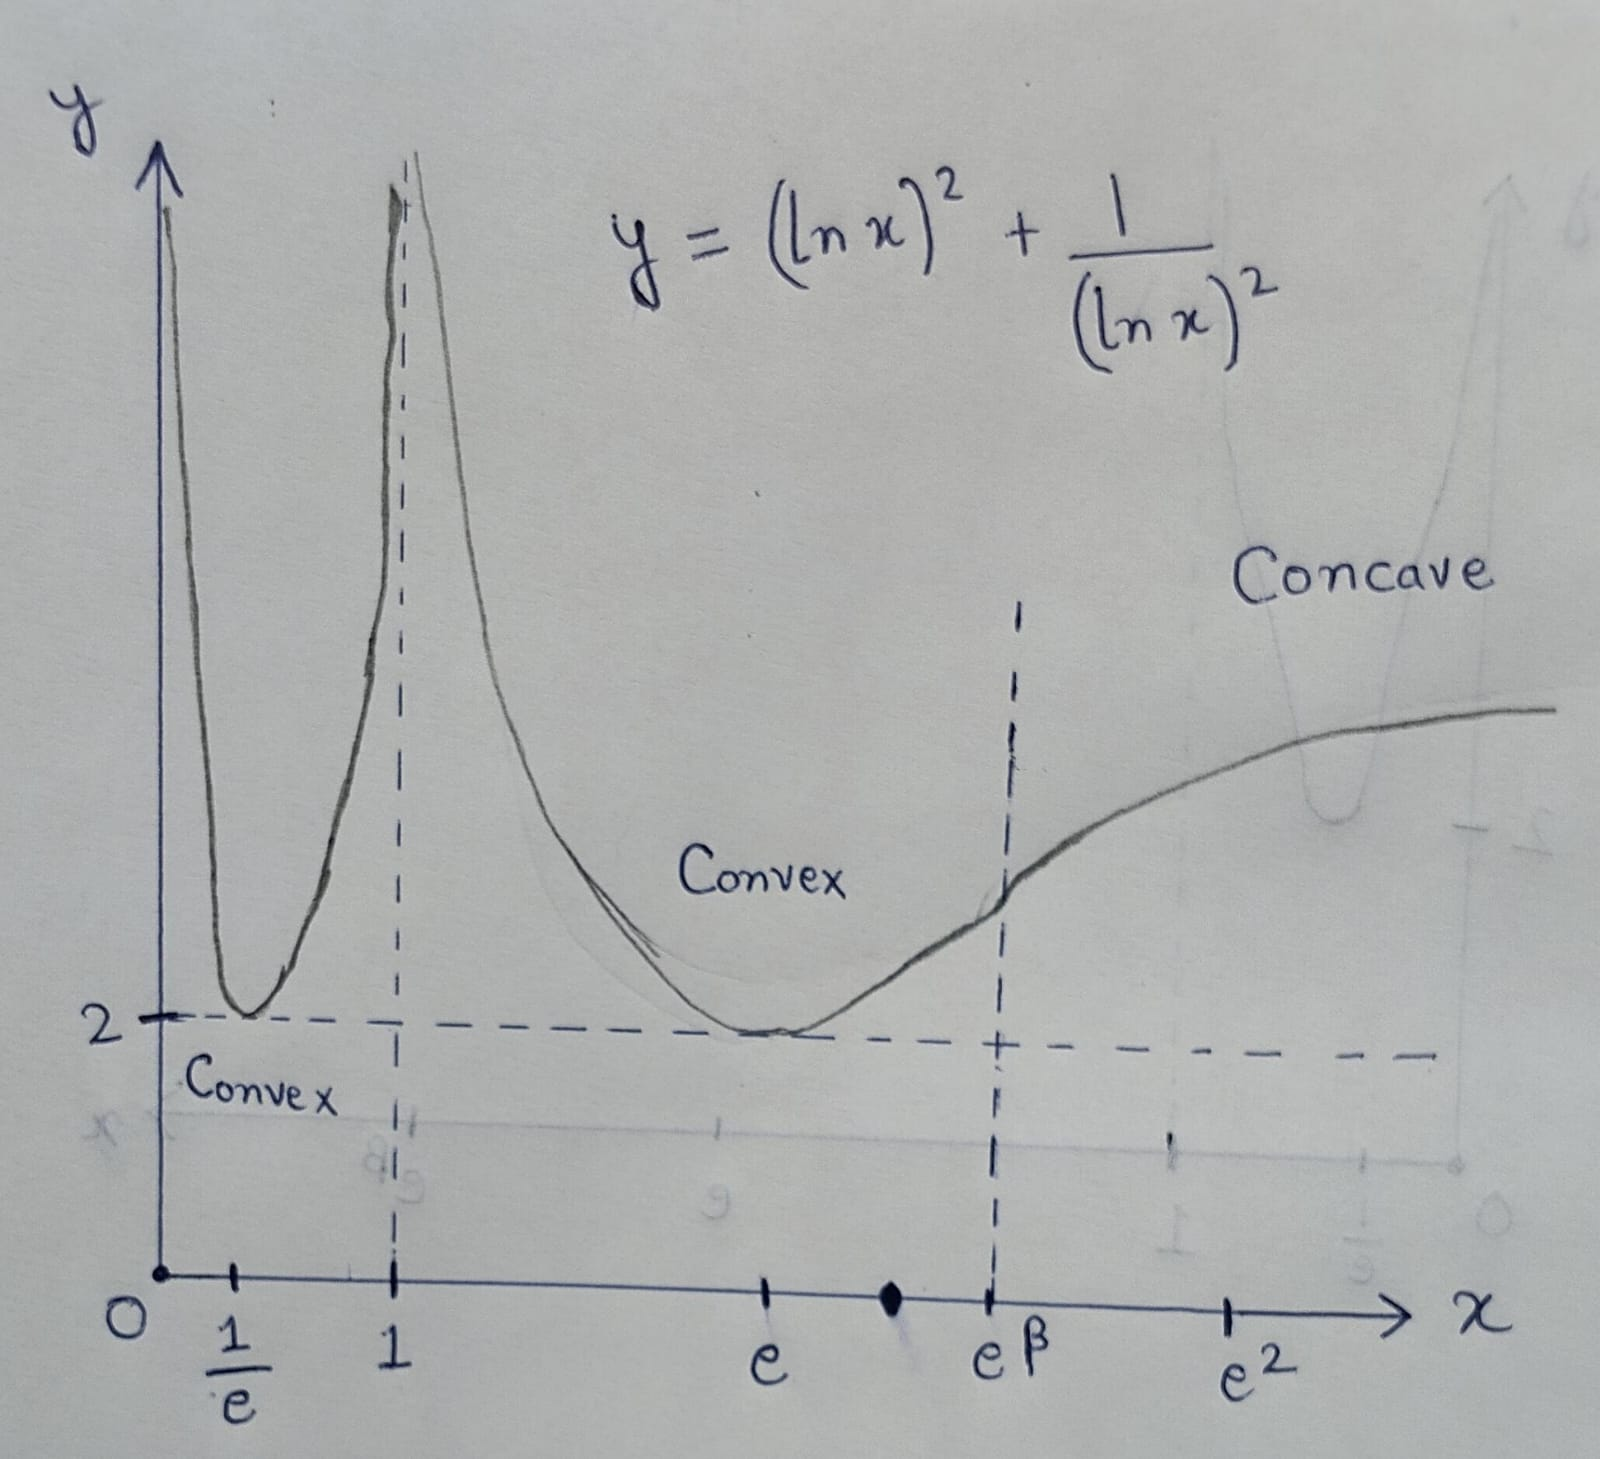
\includegraphics[scale=0.115]{../../../src/content/posts/isi_2026_discussion/final_graph_handmade.png}
            \caption{Handmade Graph of $f$}
        \end{minipage}
    \end{figure}

    \noindent This indeed \textbf{completes the solution}
    to the problem.
\end{sol}
\newpage

\section{UGB 2026/3}
\begin{prob}{(UGB 2026/3)}{}
    Suppose $n \geq 2$ is an integer. Define
    \[S = \{(x_1, \dots, x_n) : 0 < x_i < 1 \text{ for all } i = 1, \dots, n\}\]
    and a function $f\colon S \to \RR$ by
    \[f(x_1, \dots, x_n) = \log_{x_1} ((x_2)^2) + \dots + \log_{x_{n-1}} ((x_n)^n) + \log_{x_n} x_1.\]
    Determine the minimum value of
    $f(x_1, \dots, x_n)$ over $S$.
\end{prob}

\begin{sol}
    The answer is $n \sqrt[n]{n!}$. Note that
    \begin{align*}
        f(x_1,x_2,\dots,x_n) & =  \log_{x_1} ((x_2)^2) + \dots + \log_{x_{n-1}} ((x_n)^n) + \log_{x_n} x_1 \\
                             & = \left(\sum_{i = 1}^{n-1}\log_{x_i} x_{i+1}^{i+1}\right) + \log_{x_n}x_1.
    \end{align*}

    \noindent First of all note that for $a,b \in (0,1)$,
    \[ a < 1 \implies \log_{b} a > \log_b(1) = 0\]
    therefore, every summand is positive and we can
    apply AM-GM inequality.

    The following claim is crucial for applying AM-GM
    inequality later on.
    \begin{claim*}
        $\displaystyle \left(\prod_{i = 1}^{n-1}\log_{x_i} x_{i+1}^{i+1}\right) = \frac{n!}{\log_{x_n}x_1}$
        for all $n \ge 2$.
    \end{claim*}
    \begin{proof}
        The proof is by induction on $n$. For the base case
        of $n = 2$, observe that
        \[\prod_{i = 1}^{2-1} \log_{x_i}x_{i+1}^{i+1} = \log_{x_1} x_2^2 = 2! \cdot \log_{x_1}{x_2} = \frac{2!}{\log_{x_2}{x_1}} \]
        where the last equality is due a change of base
        formula to base $x_1$. This verifies the base case.
        For the \textbf{induction hypothesis}, assume that
        \[\left(\prod_{i = 1}^{m-1}\log_{x_i} x_{i+1}^{i+1}\right) = \frac{m!}{\log_{x_m}x_1}\]
        for some $m \ge 2$. We need to show that holds true
        for $m + 1$ as well. For the \textbf{induction step},
        observe
        \begin{align*}
            \prod_{i = 1}^m \log_{x_i} x_{i+1}^{i+1} & = \prod_{i = 1}^{m-1} \log_{x_i} x_{i+1}^{i+1} \cdot \left( \log_{x_m}x_{m+1}^{m+1} \right)                    \\
                                                     & = \frac{m!}{\log_{x_m}x_1} \cdot (m+1)\cdot \log_{x_m} x_{m+1} \quad \text{(By \textbf{induction hypothesis})} \\
                                                     & = (m+1)! \cdot \frac{\log_{x_m} x_{m+1}}{\log_{x_m} x_{1}} = (m+1)!\cdot \log_{x_1} x_{m+1}                    \\
                                                     & = \frac{(m+1)!}{\log_{x_{m+1}} x_1}
        \end{align*}
        where we have continuously applied change of base
        formula of logarithms. This completes the induction
        step and the proof to the claim.
    \end{proof}

    \paragraph{Proof of Lower Bound} We first Simply applying
    AM-GM Inequality to the $n$ summands yields
    \begin{align*}
        \frac{\left(\sum_{i = 1}^{n-1}\log_{x_i} x_{i+1}^{i+1}\right) + \log_{x_n}x_1}{n} & \ge \sqrt[n]{\left( \prod_{i = 1}^{n-1} \log_{x_i}x_{i+1}^{i+1} \right) \cdot \log_{x_n}x_1} \\
                                                                                          & = \sqrt[n]{\left( \frac{n!}{\log_{x_n} x_1} \right) \cdot \log_{x_n} x_1}                    \\
                                                                                          & = \sqrt[n]{n!}
    \end{align*}
    Multiplying both the sides by $n$ gives us
    \[ f(x_1,x_2,\dots, x_n) \ge n\cdot{\sqrt[n]{n!}}\]
    which is what we wanted to show.

    \paragraph{Proof of Attainability of Bound}
    We will show that the lower bound given above is
    achieved when
    \[ x_i = x_1^{\frac{n!}{i!t^{n-i+1}}} \iff \log_{x_1}x_i = \frac{n!}{i! t^{n-i+1}}\]
    for $i = 1,2,3,\dots,n$ where $t = \sqrt[n]{n!}$ where
    $x_1$ can be any real in $(0,1)$. Also, note that
    since $\frac{n!}{i! t^{n-i+1}} > 0$, we know that
    \[x_i = x_1^{\frac{n!}{i! t^{n-i+1}}} < x_1 ^ 0 = 1 \]
    which ensures $0 < x_i < 1$ for $i = 1,2,3,\dots, n$.

    We will look at every summand individually. First
    observe that
    \[ x_n = x_1^{1/t} \implies \log_{x_n}x_1 = t.\]
    For any other summand $\log_{x_i} x_{i+1}^{i+1}$
    where $1 \le i \le n-1$, observe that
    \begin{align*}
        \log_{x_i} x_{i+1}^{i+1} & = (i+1)\frac{\log_{x_1} x_{i+1}}{\log_{x_1}x_i}                     \\
                                 & = (i+1) \cdot \frac{n!}{(i+1)!t^{n-i}} \cdot \frac{i!t^{n-i+1}}{n!} \\
                                 & = t.
    \end{align*}
    So, finally
    \[ f(x_1,x_2, \dots, x_n) = \sum_{i = 1}^{n-1}\log_{x_i} x_{i+1}^{i+1} + \log_{x_n} x_1 = (n-1)t + t = nt = n\sqrt[n]{n!} \]
    which \textbf{completes the solution.}
\end{sol}
\newpage

\section{UGB 2026/4}

\begin{prob}{(UGB 2026/4)}{}
    Suppose $f\colon \RR \to \RR$ is a twice
    differentiable function such that
    \[f(x + y) + f(x - y) = 2(f(x) + f(y)) \text{ for all } x, y \in \RR.\]
    \begin{enumerate}[label=\alph*)]
        \item If $f'$ denotes the derivative of $f$,
              show that
              \[f'(x + y) - f'(x - y) = 2f'(y) \text{ for all } x, y \in \RR.\]
        \item Further assume that $f''(0) = 2$, where
              $f''$ is the second derivative of $f$.
              Determine $f$.
    \end{enumerate}
\end{prob}

\begin{sol}
    Denote the functional equation
    $f(x + y) + f(x - y) = 2\left(f(x) + f(y)\right)$ by
    $(\clubsuit)$.
    Observe that putting $x = y$ gives us
    $2f(0) = 4f(0) \implies f(0) = 0$. Putting $x = 0$
    in $(\clubsuit)$ yields
    \[ f(y) + f(-y) = 2f(y) \implies f(-y) = f(y)\,\, \text{for all\,\,} y \in \RR.\]
    which proves that $f$ is even. We will solve each part
    individually.

    \paragraph{Solution to part a)} Fix $x = x_0 \in \RR$
    in $(\clubsuit)$. Since $f$ is given to be
    differentiable(twice differentiable in fact), so we can
    differentiate both sides of $(\clubsuit)$ with respect
    to $y$. This yields
    \begin{align*}
        \frac{d}{dy} \bigg( f(x_0+y) + f(x_0-y) \bigg) & = \frac{d}{dy} \bigg(2f(x_0) + 2f(y)\bigg) \\
        \implies f'(x_0 + y) - f(x_0 - y)              & = 2f'(y)\,\, \text{for all $y \in \RR$.}
    \end{align*}
    Since $x_0$ was fixed arbitrarily, the above equation is
    also true for all $x \in \RR$. Thus, we get
    \[f'(x + y) - f'(x - y) = 2f'(y) \text{ for all } x, y \in \RR. \tag{$\spadesuit$} \label{q4-a}\]
    This \textbf{finishes the proof of part a).} \bsquare

    \paragraph{Solution to part b)} We will prove that
    $f(x) = x^2$ is the only possible $f$ satisfying
    the functional equation. As
    \[f(x+y) + f(x-y) = (x+y)^2 + (x-y)^2 = 2(x^2 + y^2) = 2\left(f(x) + f(y)\right) \]
    the claimed characteriziation indeed works. We will now
    prove that this the only possible $f$ satisfying
    $(\clubsuit)$.

    $f$ is given to be twice-differentiable, so we will
    differentiate both sides of \eqref{q4-a} with respect
    to $x$ this	time. This involves first fixing $y$
    arbitrarily like we did in \textbf{part a)}. We'll
    skip these details this time.
    \begin{align*}
        \frac{d}{dx} \bigg(f'(x+y) - f'(x-y)\bigg) & = \frac{d}{dx} \bigg( 2f'(y) \bigg)          \\
        \implies f''(x+y) - f''(x-y)               & = 0                                          \\
        \implies f''(x+y)                          & = f''(x-y) \,\,\text{for all $x,y \in \RR$.}
    \end{align*}
    Replace $x$ with $x+y$ in the above equation to get
    \[ f''(x+2y) = f''(x) \,\,\text{for all $x,y \in \RR$.}\]
    Finally, replace $y$ by $y/2$ and then put $x = 0$,
    with the fact $f''(0) = 2$(given in the problem
    statement) which gives
    \[ f''(y) = f''(0) = 2 \,\,\text{for all $y \in \RR$.}\]
    This proves that $f''$ identically $2$ on $\RR$.
    This is a very simple differential equation to solve,
    integrating both sides once gives
    \[ f'(x) = \int 2\, dx = 2x + C \,\,\text{for come constant $C \in \RR$.}\]
    Integrating once more gives
    \[f(x) = \int 2x + C \, dx = x^2 + Cx + D \,\, \text{for some constants $C,D \in \RR$.} \]
    Since $f(0) = 0$, we get $D = 0$. Using $f(x) = f(-x)$,
    we get
    \[ f(x) = x^2 + Cx = f(-x) = x^2 - Cx \implies 2Cx = 0 \,\,\text{for all $x \in \RR$.} \]
    Since $2Cx = 0$ for any $x \in \RR$, putting $x = 1$
    forces $C = 0$ which gives $f(x) = x^2$ for all
    $x \in \RR$, \textbf{completing the solution to part b)}.
\end{sol}
\newpage

\section{UGB 2026/5}
\begin{prob}{(UGB 2026/5)}{}
    In the figure below, $ABCD$ is a square. The
    points $E, F, G, H$ lie on $AB, BC, CD, DA$,
    respectively, such that $EFGH$ is a square. The
    perimeter of $ABCD$ exceeds the perimeter of
    $EFGH$ by 32 units. Determine the length of the
    radius of the in-circle of $\Delta EBF$.

    \centering
    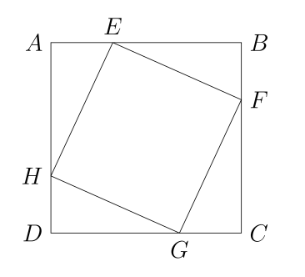
\includegraphics[trim=0 17 0 0, clip, scale=0.5]{../../../src/content/posts/isi_2026_discussion/geo_question.png}
\end{prob}
\begin{sol}
    The answer is 4 units. Let the side-length of square
    $ABCD$ be $y$ and the side-length of square $EFGH$ be
    $x$. By the given perimeter condition,
    \[4y = 4x + 32 \implies y = x + 8. \]

    \noindent We will now prove the following important claim.
    \begin{claim*}
        $\displaystyle \triangle EFB \cong \triangle HEA \cong \triangle GHD \cong \triangle FGC.$
    \end{claim*}
    \begin{proof}
        Let $\theta \coloneqq \angle BEF$, then
        \[\angle AEH = 180\dg - (\angle HEA + \angle BEF) = 180\dg - (90\dg + \theta) = 90\dg - \theta. \]
        \begin{center}
            \begin{asy}
                import olympiad;
                size(150);
                defaultpen(fontsize(13pt));
                pair A, B, C, D, E, F, G, H;

                real L = 49;
                real x = 9;

                A = (0,L);
                B = (L,L);
                C = (L,0);
                D = (0,0);

                E = (x,L);
                F = (L,L-x);
                G = (L-x, 0);
                H = (0, x);

                draw(A--B--C--D--cycle);
                draw(E--F--G--H--cycle);

                dot("$A$", A, dir(135));
                dot("$B$", B, dir(45));
                dot("$C$", C, dir(315));
                dot("$D$", D, dir(225));
                dot("$E$", E, dir(90));
                dot("$F$", F);
                dot("$G$", G, dir(270));
                dot("$H$", H, W);

                draw(E--B--F--cycle);
                draw(incircle(E,F,B));

                label("$\theta$", E, dir(354)*12);
                label("$\theta$", H, dir(83.5)*10);

                markscalefactor = 0.3;
                draw(rightanglemark(F,C,G), deepgreen);
                draw(rightanglemark(H,E,F), deepgreen);
                draw(rightanglemark(H,A,E), deepgreen);

                markscalefactor = 1.3;
                draw(anglemark(F,E,B));
                draw(anglemark(E,H,A));
            \end{asy}
        \end{center}
        By angle sum in $\triangle AEH$, $\angle AHE = \theta$.
        Note that $\ol{HE} = \ol{EF}$(equal sides of square
        $EFGH$), $\angle HAE = \angle EBF = 90\dg$ and
        $\angle BEF= \angle AHE = \theta$, so by AAS
        criteria $\triangle EFB \cong HEA$. The other
        congruencies can be proven in a similar fashion. This
        \textbf{proves our claim.}
    \end{proof}

    The corresponding parts of the congruent triangles yield
    $\ol{BF} = \ol{AE}$. From here, we will present two finishes
    to this problem.

    \paragraph{First Finish, Direct Formula} We prove the
    well-known theorem for inradius of a right triangle.
    \begin{theorem*}[Inradius of Right Triangle]
        Denote the inradius of $\triangle EBF$ right-angled
        at $B$ by $r$, then
        \[ r = \frac{f+e-b}{2}\]
        where $f = \ol{EB}$, $e = \ol{BF}$ and $b = \ol{EF}$
    \end{theorem*}
    \begin{proof}
        If $I$ is incenter of $\triangle EBF$, then let
        $X,Y,Z$ be feet of perpendiculars from $I$ to
        $BF$, $EB$ and $FE$ respectively.

        \begin{center}
            \begin{asy}
                import olympiad;
                size(280);
                defaultpen(fontsize(13pt));

                pair B = (0,0);
                pair F = (0,9);
                pair E = (40,0);

                pair I = incenter(B,E,F);
                pair X = foot(I,B,F);
                pair Y = foot(I,E,B);
                pair Z = foot(I,F,E);

                draw(E--B--F--cycle);
                draw(incircle(B,E,F));
                draw(I--X); draw(I--Y); draw(I--Z);

                dot("$E$", E, dir(E));
                dot("$F$", F, dir(F));
                dot("$B$", B, dir(180));
                dot("$I$", I, dir(I));

                dot("$X$", X, dir(180));
                dot("$Y$", Y, dir(270));
                dot("$Z$", Z, dir(Z));
            \end{asy}
        \end{center}
        Since $\angle IYB = \angle IXB =\angle XBY = 90\dg$,
        so we by angle sum of quadrilateral $IXBY$, we get
        $\angle XIY = 90\dg$ which tells us $IXBY$ is a
        rectangle. Moreover, $IXBY$ is a square since
        $\ol{IX} = \ol{IY}$. Finally,
        \[b = \ol{FE} = \ol{EZ} + \ol{ZF} = \ol{EY} + \ol{FX} = (f-r) + (e-r) \implies r = \frac{f+e-b}{2} \]
        where we used $\ol{EZ} = \ol{EY}$ and
        $\ol{FZ} = \ol{FX}$ since length of tangents drawn
        from an external point are equal The
        \textbf{proof to the theorem is now complete.}
    \end{proof}

    To conclude note that
    \[r = \frac{f + e - b}{2} = \frac{\ol{BE} + \ol{BF}-\ol{FE}}{2} = \frac{\ol{BE} + \ol{AE} - x}{2} = \frac{\ol{AB}-x}{2} = \frac{x + 8 - x}{2} = 4 \]
    which \textbf{finishes the first solution.} \bsquare

    \paragraph{Second Finish, Algebraic} Retain all the
    notation from previous solution. We'll use the
    more standard formula,
    \[ r = \frac{\Delta}{s}\]
    where $\Delta$ and $s$ is the area and semi-perimeter
    of $\triangle EBF$. We know $\Delta = \half \cdot ef$
    and $s = \half \cdot (e + b + f)$. Simplifying we get
    \[r = \frac{fe}{f + e + b} \]
    We know that
    \[f + e + b = \ol{BE} + \ol{BF} + b = \ol{BE} + \ol{AE} +b = \ol{AB} + b = x + 8 + x = 2x + 8.\]
    By Pythagoras Theorem on $\triangle EBF$, we get
    $f^2 + e^2 = b^2 = x^2$. This gives
    \[fe = \frac{(f+e)^2 - e^2 - f^2}{2} = \frac{(x+8)^2-x^2} {2} = 8x + 32 \]
    Finally,
    \[r = \frac{fe}{f + e + b} = \frac{8x+32}{2x + 8} = \frac{8\cancel{(x+4)}}{2\cancel{(x+4)}} = 4 \]
    and \textbf{we're done.}
\end{sol}
\newpage

\section{UGB 2026/6}

\begin{prob}{(UGB 2026/6)}{}
    Let $P$ be a polynomial of degree greater than or
    equal to one, with real coefficients, such that
    $P(x) \geq 0$ for all $x \in \RR$.
    \begin{enumerate}[label=\alph*)]
        \item Suppose $x_0 \in \RR$ is such that
              $P(x_0) = 0$. Show that there exist a
              positive integer $n$ and a polynomial
              $S$ with real coefficients such that
              $S(x_0) \neq 0$ and
              \[P(x) = (x - x_0)^{2n} S(x) \text{ for all } x \in \RR.\]
        \item Hence or otherwise, show that there
              exist polynomials $Q$ and $R$ with real
              coefficients such that $R(x) > 0$ for
              all $x \in \RR$ and
              \[P(x) = (Q(x))^2 R(x) \text{ for all } x \in \RR.\]
    \end{enumerate}
\end{prob}

\begin{sol}
    We first prove a well-known preparatory lemma.
    A root $\alpha$ of $P$ is said to be a repeated root
    of $P$ if its multipilicity is at least $2$.

    \begin{lemma*}[Repeated Roots]
        Let $\alpha$ be a root of the polynomial $P$,
        then $\alpha$ is a repeated root of
        $P \iff P'(\alpha) = 0$.
    \end{lemma*}
    \begin{proof}
        Suppose first that $\alpha$ is a repeated root of
        $P$. Then
        \[ P(x)=(x-\alpha)^2Q(x) \]
        for some polynomial $Q$. Differentiating, we
        obtain
        \[ P'(x)=2(x-\alpha)Q(x)+(x-\alpha)^2Q'(x).\]
        Evaluating at $x=\alpha$ yields $P'(\alpha)=0$.

        Conversely, suppose that $P'(\alpha)=0$. Since
        $\alpha$ is a root of $P$, by the Factor Theorem,
        $P(x)=(x-\alpha)Q(x)$ for some polynomial $Q$.
        Differentiating gives
        \[
            P'(x)=Q(x)+(x-\alpha)Q'(x).
        \]
        Evaluating at $x=\alpha$, we find that
        $Q(\alpha)=P'(\alpha)=0$.
        Applying the Factor Theorem once again, we conclude that
        $(x-\alpha)$ divides $Q(x)$. Hence
        \[
            P(x)=(x-\alpha)^2R(x)
        \]
        for some polynomial $R$, showing that $\alpha$ is a repeated root
        of $P$.
    \end{proof}

    First of all observe that $\deg(P)$ must be even
    because all odd degree polynomials have range $\RR$,
    thus we only need to prove the hypothesis for
    even degree polynomials $P$. We will solve
    both the parts with induction, but on different
    variables.

    \paragraph{Solution to part a)} We prove the
    following claim.

    \begin{claim*}
        $x_0$ is a repeated root of $P$.
    \end{claim*}
    \begin{proof}
        Since $x_0$ is given to be a root of $P$, by the
        lemma proven above, it suffices to prove
        $P'(x_0) = 0$. For any $h > 0$,
        $P(x_0 + h) - P(x_0) = P(x_0 + h) \ge 0$, which
        means that
        \[\text{RHD}_{x_0} = \lim_{h \to 0^+} \frac{P(x_0+h) - P(x_0)}{h} \ge 0 \]
        where RHD$_{x_0}$ means the right-hand derivative
        at $x_0$. For any $h > 0$,
        $P(x_0 - h) - P(x_0) = P(x_0 - h) \ge 0$. Now,
        \[\text{LHD}_{x_0} = \lim_{h \to 0^+} \frac{P(x_0-h) - P(x_0)}{-h} \le 0 \]
        where LHD$_{x_0}$ means the left-hand derivative
        at $x_0$.

        Recall that polynomials are differentiable
        everywhere, so $P$ must be differentiable at $x_0$.
        Also, $P$ is differentiable at $x_0$ if and only if
        the LHD$_{x_0}$ = RHD$_{x_0}$. This means
        \[ 0 \le \text{RHD}_{x_0} = \text{LHD}_{x_0} \le 0 \implies \text{RHD}_{x_0} = \text{LHD}_{x_0} = 0 \implies P'(x_0) = 0 \]
        which proves our claim.
    \end{proof}

    We will now solve the problem by induction, by
    inducting on the degree of $P$.

    \begin{claim*}[Essentially part a]
        Any non-negative even degree polynomial $P$ if
        posesses a root $x_0$ must have an even
        multiplicity.
    \end{claim*}
    \begin{proof}
        As advertised earlier, we will prove this by
        induction on $\deg(P)$. So let $\deg(P) = 2d$.
        We will first deal with the base of $d = 1$.
        Thus we need to show that if $x_0$ is the root
        of the quadratic
        $ax^2 + bx + c$($a$, $b$, $c \in \RR)$, then
        $\alpha$ is a double root of $P$. By the
        \emph{Factor Theorem}, we can write
        \[ ax^2 + bx + c = (x-x_0)(ux + v) \]
        where $u,v$ are some real constants. Any quadratic
        polynomial with two distinct roots \textbf{can NOT}
        be non-negative. This is easy to see, if
        $R(x) = r(x-\alpha)(x-\beta)$, then $R$ either
        negative on the interval
        $\big( \min(\alpha,\beta), \max(\alpha, \beta) \big)$
        (based upon the sign of $r$).
        Thus $ux + v$ must have $x_0$ as a root. This
        resolves the base case.

        As an \textbf{induction hypothesis}, assume that
        all non-negative polynomials with degree $2d'$,
        if possess a root $x_0$, then multiplicity of
        $x_0$ is always even.

        For the \textbf{induction step}, we wish to
        show that all non-negative polynomials of degree
        $2(d'+1) = 2d' + 2$	with root $x_0$, posseses
        $x_0$ as a root with even multiplicity. So, let
        $Q$ be an arbitrary non-negative polynomial with
        $\deg(Q') = 2d' + 2$ with root $x_0$. By the
        claim proven above, we know $x_0$ is a repeated
        root. Therefore, we can write
        \[Q(x) = (x-x_0)^2 T(x) \]
        where $\deg(T) = 2d'$. If $x_0$ is \textbf{NOT} a
        root of $T$, then we are done. If $x_0$ is a root
        of $T$, then by the \textbf{induction hypothesis}(the
        hypothesis applies since $\deg(T)$ is even and
        $T(x) = Q(x)/(x-x_0)^2 \ge 0$),
        $T$ must possess $x_0$ as a root with an even
        multiplicity. So, we can write
        $T(x) = (x-x_0)^{2m}U(x)$ where $U(x_0) \ne 0$.
        This gives
        \[Q(x) = (x-x_0)^{2m+2} S(x) \]
        with $S(x_0) \ne 0$. This proves the claim.
    \end{proof}

    \noindent The above claim essentially
    \textbf{finishes the proof to part a).} \bsquare

    \paragraph{Solution to part b)} The proof is once again
    by induction, but we will use strong induction this time.

    \begin{claim*}[Essentially part b]
        All non-negative even degree polynomials $P$ with
        $\deg(P) = 2d$ can be written as
        \[ P(x) = Q(x)^2\cdot R(x)\]
        with $R > 0$.
    \end{claim*}
    \begin{proof}
        We will strong induct on $d$. The base case $d = 1$,
        wants us to show that any non-negative quadratic
        polynomial $P$ can be written in the form
        $Q(x)^2\cdot R(x)$. If $P$ doesn't have have any
        root, then $P > 0$. Then we can pick $Q(x) = 1$
        and $R = P$. If $x_0$ is a root of $P$, then
        by \textbf{part a)}, we know that $x_0$ is a double
        root. Therefore,
        \[P(x) = a(x-x_0)^2 \]
        where $a > 0$. So, here picking $Q(x) = x-x_0$ and
        $R(x) = a$ works.

        As an \textbf{induction hypothesis}, assume that
        all non-negative polynomials $P$ of degree
        $2k$ where $k = 1,2,\dots, d'$ can be written in the
        form $Q(x)^2R(x)$ where $R > 0$.

        For the \textbf{induction step}, we need to show
        that any non-negative polynomial $T$ with
        $\deg(P) = 2(d'+1) = 2d'+2$ can also be written in
        the form $Q(x)^2R(x)$. If $T$ doesn't have a root,
        then picking $Q(x) = 1$ and $R(x) = 1$ is enough.

        If $T$ has a root $\alpha$, then by \textbf{part a)},
        \[ T(x) = (x-x_0)^{2m}U(x)\]
        with $U(x_0) \ne 0$. Clearly $\deg(U)$ is even
        and $U \ge 0$, so applying the \textbf{induction
            hypothesis} tells us that there exists polynomials
        $A,B \in \RR[x]$ such that $U(x) = A(x)^2\cdot B(x)$
        with $B > 0$. This yields
        \[ T(x) = (x-x_0)^{2m}\cdot A(x)^2\cdot B(x) = \big((x-x_0)^m\cdot A(x)\big)^2\cdot B(x)\]
        Picking $Q(x) = (x-x_0)^m\cdot A(x)$ and $R = B$
        completes the strong induction.
    \end{proof}

    \noindent This \textbf{completes the solution to
        part b)} and the concludes the entire solution.
\end{sol}
\newpage

\section{UGB 2026/7}

\begin{prob*}{(UGB 2026/7)}{}
    Suppose $P$ is a polynomial with integer coefficients.
    \begin{enumerate}[label=\alph*)]
        \item Show that for distinct integers $m$ and
              $n$, $\frac{P(m) - P(n)}{m - n}$ is an
              integer.
        \item Hence or otherwise, prove that there do
              not exist distinct integers $a, b, c$
              such that
              \[P(a) = b, \quad P(b) = c, \quad \text{and} \quad P(c) = a.\]
    \end{enumerate}
\end{prob*}

\begin{sol}
    We will split the solution into two parts.

    \paragraph{Solution to part a)} Write
    \[ P(x) = \sum_{i = 0}^d a_i x^i \]
    where $a_i \in \ZZ$ for $i = 0,1,\dots, d$. Since
    $a_i\cdot m^i \in \ZZ$ for any $m \in \ZZ$ and
    $m - n \in \ZZ$, the problem statement is equivalent
    to showing $m-n \mid P(m) - P(n)$. For distinct
    integers $m,n$
    \[P(m) - P(n) = \sum_{i = 0}^d a_i(m^i - n^i) = \sum_{i = 1}^d a_i(m^i - n^i) \]
    since $a_0(m^0 - n^0) = 0$. Recall the following
    standard lemma.
    \begin{lemma*}[Standard Divisibility]
        Given $m,n \in \ZZ$, $m - n \mid m^k - n^k$ for
        all $k \in \ZZ_{\ge 1}$.
    \end{lemma*}
    \begin{proof}
        We shall strong induct on $k$. The base case of
        $k = 1$ is trivial. As an
        \textbf{induction hypothesis}, assume that
        $m-n \mid m^t - n^t$ for $t = 1,2,\dots, k$ for
        $k \ge 1$. For the \textbf{induction step}, we need
        to show $m - n \mid m^{k + 1} - n^{k + 1}$. By the
        \textbf{induction hypothesis}, we know that
        \begin{align*}
            m - n \mid m^k - n^k & \implies m - n \mid m(m^k - n^k) = m^{k+1} -mn^k \\
            m - n \mid m^k - n^k & \implies m - n \mid m(m^k - n^k) = nm^k -n^{k+1}
        \end{align*}
        Adding both the division relations we get
        \[m - n \mid m^{k+1} - n^{k+1} -mn(m^{k-1} - n^{k-1}) \]
        By our \emph{strong} \textbf{induction hypothesis},
        $m - n \mid m^{k-1} - n^{k-1}$, which ultimately
        gives
        \[ m - n \mid m^{k+1} - n^{k+1} \]
        completing the \textbf{induction step} and the
        proof of the lemma.
    \end{proof}

    Due to the above lemma, we can now write
    $m^k - n^k = (m-n)q_k$ where $q_k \in \ZZ$ and $q_k$ is
    dependent upon $k$ where $k \ge 1$. Thus,
    \[P(m) - P(n) = \sum_{i = 1}^d a_i(m^i - n^i) = \sum_{i = 1}^d a_i\cdot q_i(m-n) = (m-n)\cdot \left(\sum_{i = 1}^d a_iq_i\right) \]
    Since $a_i,q_i$ are integers for $i = 1,2,\dots, d$,
    $\sum a_iq_i \in \ZZ$ as well. This gives
    $m - n \mid P(m) - P(n)$ which finishes the
    \textbf{proof to part a).} \bsquare
    \paragraph{Solution to part b)} Assume for the sake
    of contradiction that there exists distinct $a$, $b$
    and $c$ satisfying
    \[P(a) = b, \quad P(b) = c, \quad \text{and} \quad P(c) = a.\]
    With the help of \textbf{part a)}, we now know that
    \[ a - b \mid P(a) - P(b) = b - c. \]

    Similarly with $b - c \mid P(b) - P(c)$ and
    $c - a \mid P(c) - P(a)$, we will get the following
    division relations. This gives
    \begin{align*}
        a - b & \mid b - c \\
        b - c & \mid c - a \\
        c - a & \mid a - b
    \end{align*}

    We now prove a short standard lemma.
    \begin{lemma*}[Divisibility Inequality]
        For $x,y \in \ZZ$ where $x,y \ne 0$ and $x \mid y$
        then
        \[ |y| \ge |x|. \]
    \end{lemma*}
    \begin{proof}
        Since $x \mid y$, there exists some $k \in \ZZ$ such
        that $kx = y$. If $k = 0$, then $y = 0$
        contradiction. Thus $|k| \ge 1$ and finally
        \[1 \le |k| = \frac{|y|}{|x|} \implies |x| \le |y|. \qedhere\]
    \end{proof}

    Clearly, none of $a-b, b-c, c-a$ none of them are
    $0$, otherwise we get contradiction on distinct nature
    of $a,b,c$. Note that
    \[ a - b \mid b-c \mid c-a \mid a-b. \]
    Applying the lemma, we get
    \[ |a-b| \le |b-c| \le |c-a| \le |a-b| \implies |a-b| = |b-c| = |c-a|.\]
    We have $|a-b| = |b-c| \implies a-b = \pm (b-c)$.
    If $a-b = -(b-c)$, then $a = c$, a contradiction since
    $a$, $b$ and $c$ are distinct. Therefore,
    $a-b = b-c \implies 2b = a + c$. Similar reasoning
    on $|a - b| = |c - a|$ and $|b-c| = |c-a|$ gives
    us the following system.
    \begin{align*}
        2c & = a + b \\
        2a & = b + c \\
        2b & = a + c
    \end{align*}
    Subtract the first two equations to get
    $2c - 2a = a - c \implies 3c = 3a \implies c = a$ which
    is again a contradiction. This
    \textbf{completes the the solution to part b).}
\end{sol}
\newpage

\section{UGB 2026/8}
\begin{prob*}{(UGB 2026/8)}{}
    Let $k$ be a non-negative integer.
    \begin{enumerate}
        \item Show that there exists a unique
              polynomial $P_k$ of degree $k+1$ with
              real coefficients such that
              \[\sum_{i=1}^{n} i^k = P_k(n) \text{ for all } n \geq 1.\]
        \item Determine the coefficient of
              $x^{k+1}$ in $P_k(x)$.
        \item Hence or otherwise, determine the
              coefficient of $x^k$ in $P_k(x)$.
    \end{enumerate}
\end{prob*}
\begin{sol}
	To be added\dots For now, the informal solution is
	available on the blog
	\begin{center}
		\small
		\url{https://satisfiedmagma.github.io/writings/posts/isi_2026_discussion/#-problem-8}
	\end{center}
	\textbf{Thank you!}
\end{sol}
\newpage

\section{Concluding Remarks}
I pretty much have summed up everything on the blog.
Although, I would like to mention that maybe the problems 
were on the easier side and a skilled candidate would 
have a really easy time, but once again the entrance 
paper has a lot of room to make error even in the simpler 
problems. Proof-writing is going to make the major difference
for the people who reach the Merit List!

I hope you enjoyed reading the solutions and 
learnt something new from them. It was my very
first blog on my website and I've tried my best. This is 
Magma, signing off ;)
\end{document}
